\documentclass{article}
\usepackage[utf8]{inputenc}
\usepackage[T1]{fontenc}
\usepackage{amsmath}
\usepackage{amsfonts}
\usepackage{amssymb}
\usepackage{amssymb, bm}
\usepackage{mathtools, bm}
\usepackage{mathrsfs}
\usepackage{stmaryrd}
\usepackage{graphicx}
\usepackage{tikz}
%\usepackage[]{algorithm2e}
\usepackage[]{algorithm}
\usepackage[]{algorithmic}
\usepackage{framed}

% fonction pour définir une fonction 
\newcommand{\fonction}[5]{
    \begin{array}{ccccc}
#1 & : & #2 & \to & #3\\
    & & #4 & \mapsto & #5\\ 
	\end{array}
}
\renewcommand{\contentsname}{Table des matières}
\begin{document}

\title{
    {\Large\textbf{Résolution de Formules Booléennes Quantifiées\\à l'aide de Réseaux de Neurones}}\\
	{\large Université Paris-Diderot}
}
\author{
	{Mohammed Younes Megrini}\\
	{Nicolas Nalpon}
}
\date{6 juin 2016}
\maketitle
\newpage

\tableofcontents
\newpage

\tableofcontents
\newpage

\section{Introduction}
Il y a 20 ans, Deep Blue, un programme développé par IBM, remportait une victoire historique aux échecs contre Garry Kasparov, le champion mondiale d'échecs à l'époque. En mars 2016, AlphaGo, développé par Google Deepmind, vient de remporter une victoire au jeu de Go contre Lee Sedol, l'un des meilleurs joueurs de Go au monde. Le jeu de Go est considéré comme un défi majeure de l'intelligence artificielle et cette victoire témoigne d'avancées très prometteuses.

Au cœur d'AlphaGo, l'apprentissage profond est la technologie qui est en phase de révolutionner le domaine de l'intelligence artificielle. Faisant partie de la catégorie des algorithmes évolutifs et, plus particulièrement, des algorithmes d'apprentissage automatique, l'apprentissage profond consiste à optimiser progressivement une succession de transformations non-linéaires des données afin de résoudre des problèmes d'analyse et de classification. Grâce à cette approche, on arrive à développer des algorithmes de classification (reconnaissance faciale et vocale, vision par ordinateur, reconnaissance d'écriture manuscrite...) ou de décision (AlphaGo pour le jeu de Go, Deep Q-Learner pour les jeux Atari...).\\

Notre projet consiste à utiliser l'apprentissage profond pour développer une méthode heuristique de traiter le problème de la satisfaisabilité des formules booléennes quantifiées (dit QBF-SAT) qui est une généralisation du problème de satisfaisabilité booléenne (dit SAT). Nous nous limiterons aux formules normales conjonctives prénexes suivant le format standard QDimacs.

Comme il est possible de voir une formule booléenne quantifiée comme un jeu à deux adversaires et que l'existence d'une stratégie gagnante pour l'un des deux joueurs détermine la valeur de vérité de la formule, notre algorithme consistera à faire s'affronter les deux stratégies opposées, en les améliorant progressivement, de sorte à en déduire la valeur de vérité de la formule.\\

Dans ce rapport, nous allons premièrement décrire le fonctionnement des réseaux de neurones et du processus d'apprentissage et les illustrer par un exemple théorique simple. Ensuite, on décrira en détail le fonctionnement de l'algorithme présenté plus haut.
\newpage

\section{Les Réseaux de Neurones}
Le premier modèle mathématique et informatique du neurone biologique a été donné par Warren McCulloh et Walter Pitts en 1943.
Ce modèle inspiré de la neurobiologie, fait intervenir n entrées auxquelles des fonctions sont appliquées afin d'obtenir une sortie.
Voici une définition plus formelle de ce modèle qu'on nomme: Modèle de McCulloh-Pitts     

\subsection{Définition: Modèle de McCulloh-Pitts}
	Soit la fonction  

	\[\fonction{\varphi}{\mathbb{R}^n}{\left\{0,1\right\}}{(x_1,....,x_n)}{\varphi(x_1,....,x_n)} \]

	telle que  
	\[\varphi (x_1,...,x_n) = g(f(x_1,....,x_n)). \]  

	\begin{enumerate}
		\item $f$ est définie comme étant la fonction somme 
		\[\fonction{f}{\mathbb{R}^n}{\mathbb{R}}{(x_1,....,x_n)}{\sum_{i=1}^{n} {x_i}} \] 
		\item On appelle $g$ la fonction d'activation à seuil. Celle-ci est définie de la manière suivante :

		\[g(x) = \begin{cases} 0 &\mbox{Si } x < \theta \\
				 1 & \mbox{Si } x \geq \theta
	 		 \end{cases} 
		\]
	\end{enumerate}

%**************************************************************************************% 
% code pour la figure 2

\vfill
\begin{center}
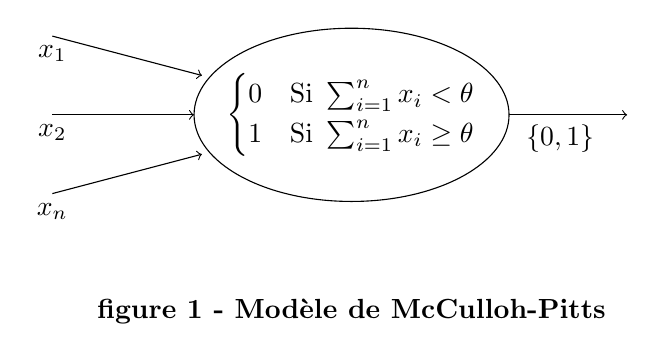
\begin{tikzpicture}[]
	%\draw[help lines, thick] (0,0) grid (9,5);
	\draw[->] (0.7,2.5) node [below] {$x_{2}$}-- (2.5,2.5);
	\draw[->] (6.5,2.5)-- node[below, align=center] {$\left\{0,1\right\}$} (7.8,2.5)-- (8,2.5);
	\draw[->] (0.7,3.5) node [below] {$x_{1}$} -- (2.6,3);
	\draw[->] (0.7,1.5) node [below] {$x_{n}$}-- (2.6,2);
	\draw (4.5,2.5) node {$ \begin{cases} 0 &\mbox{Si } \sum_{i=1}^{n} {x_i} < \theta \\ 1 & \mbox{Si } \sum_{i=1}^{n} {x_i} \geq \theta \end{cases} $} circle [x radius= 2, y radius=1.1];
	\draw (4.5,0) node { \textbf{figure 1 - Modèle de McCulloh-Pitts} };
\end{tikzpicture}
\end{center}
\vfill
%**************************************************************************************% 

\textbf{Remarque} : La valeur $\theta$  qu'on utilise dans la fonction $g$ est appelée le seuil.\\
	

Le modèle de McCulloh-Pitts a été décliné de plusieurs manières au cours du temps. Les deux déclinaisons auxquelles nous allons nous intéresser sont appelées le modèle Perceptron et le modèle sigmoïde. Ces deux modèles introduisent la notion de poids qui est au cœur du processus d'apprentissage d'un réseau de neurone. 

\subsection{Définition: Modèle Perceptron}
		Le premier modèle du Perceptron a été introduit en 1958 par Frank Rosenblatt. Celui-ci a ensuite été repris et perfectionné dans les années soixante par Minsky et Papert. Ce modèle reprend la définition précédente sauf que pour chaque entrées $x_i$ ($i$ $\in$ $\llbracket 1~;~n \rrbracket$) on associe une valeur (les fameux poids) $w_i$ $\in$ $\mathbb{R}$. 
		On définit alors la fonction $f$ de la façon suivante : 
		
		\[\fonction{f}{\mathbb{R}^n}{\mathbb{R}}{(x_1,....x_n)}{\sum_{i=1}^{n} {w_ix_i}}. \]

	
	\textbf{Remarque} : On note parfois \[b = -\theta \]  et on appel cette valeur l'inclinaison (\textit{bias} en anglais). La fonction $g$ est alors définie de la manière suivante :   
		\[g(x) = \begin{cases} 0 &\mbox{Si } x + b < 0 \\
				 1 & \mbox{Si } x + b \geq 0
	 		 \end{cases} \] \\
%**************************************************************************************% 
% code pour la figure 2
\vfill
\begin{center}
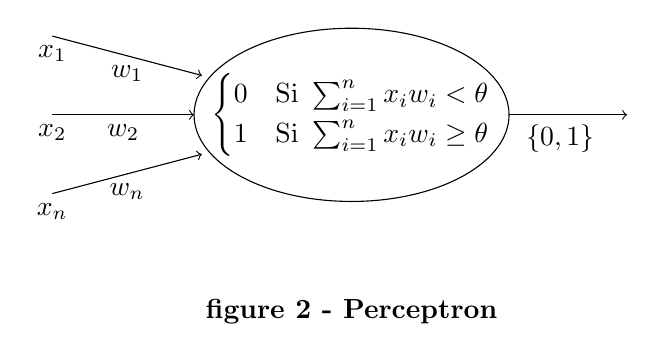
\begin{tikzpicture}[]
	%\draw[help lines, thick] (0,0) grid (9,5);
	\draw[->] (0.7,2.5) node [below] {$x_{2}$}-- node [below] {$w_{2}$} (2.5,2.5);
	\draw[->] (6.5,2.5)-- node[below, align=center] {$\left\{0,1\right\}$} (7.8,2.5)-- (8,2.5);
	\draw[->] (0.7,3.5) node [below] {$x_{1}$} -- node [below] {$w_{1}$} (2.6,3);
	\draw[->] (0.7,1.5) node [below] {$x_{n}$}-- node [below] {$w_{n}$} (2.6,2);
	\draw (4.5,2.5) node {$ \begin{cases} 0 &\mbox{Si } \sum_{i=1}^{n} {x_iw_i} < \theta \\ 1 & \mbox{Si } \sum_{i=1}^{n} {x_iw_i} \geq \theta \end{cases} $} circle [x radius= 2, y radius=1.1];
	\draw (4.5,0) node { \textbf{figure 2 - Perceptron} };
\end{tikzpicture}
\end{center}
\vfill
%**************************************************************************************% 
	 
Cette notion de poids va intervenir dans le processus d'apprentissage d'un réseau de neurone. Le but de ce processus sera d'optimiser les poids associés aux neurones afin que le réseau de neurone produise la meilleure sortie possible. L'un des algorithmes d'optimisation le plus utilisé est l'algorithme de la descente de gradient. Nous détaillerons plus tard cet algorithme mais le principe de celui-ci est d'ajuster progressivement les poids afin d'affiner la sortie du réseau de neurone vers la valeur voulue. Cet affinement implique que la sortie $s$ $\in$ $\left[0,1\right]$ et que la fonction $g$ ne soit plus une fonction en escalier mais une fonction continue. Le neurone Perceptron ne répondant pas à ces critères, le neurone Sigmoïde a été introduit. \\
% préciser le fait que avec une fonction en escalier il y a des gros saut et qu'avec une fonction continue il y a des petits sauts
% la particularitée ???
	\subsection{Définition: Modèle sigmoïde}
	 Le modèle sigmoïde est défini de la même manière que le modèle Perceptron mais avec une fonction $g$ différente. La fonction $g$ aura pour particularité d'être continue. La fonction choisie est la fonction sigmoïde.  
		  \[ \fonction{g}{\mathbb{R}}{\left[0,1\right]}{x}{ \frac{1}{1+ e^{-x}}} \]


%**************************************************************************************% 
% code pour la figure 3 
%\vfill
\begin{center}
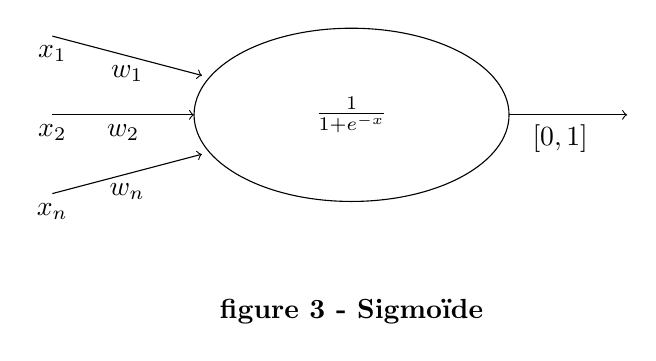
\begin{tikzpicture}[]
	%\draw[help lines, thick] (0,0) grid (9,5);
	\draw[->] (0.7,2.5) node [below] {$x_{2}$}-- node [below] {$w_{2}$} (2.5,2.5);
	\draw[->] (6.5,2.5)-- node[below, align=center] {$\left[0,1\right]$} (7.8,2.5)-- (8,2.5);
	\draw[->] (0.7,3.5) node [below] {$x_{1}$} -- node [below] {$w_{1}$} (2.6,3);
	\draw[->] (0.7,1.5) node [below] {$x_{n}$}-- node [below] {$w_{n}$} (2.6,2);
	\draw (4.5,2.5) node {$ \frac{1}{1+e^{-x}}  $} circle [x radius= 2, y radius=1.1];
	\draw (4.5,0) node { \textbf{figure 3 - Sigmoïde} };
\end{tikzpicture}
\end{center}
%\vfill
%**************************************************************************************% 
		
	\subsection{Définition: Réseau de Neurone}
 	Un réseau de neurone est un graphe orienté connexe dont les nœuds sont les neurones.\\

\def\layersep{2.5cm}
\begin{center}
\begin{tikzpicture}[shorten >=1pt,->,draw=black!50, node distance=\layersep]
    \tikzstyle{every pin edge}=[<-,shorten <=1pt]
    \tikzstyle{neuron}=[circle,fill=black!25,minimum size=17pt,inner sep=0pt]
    \tikzstyle{input neuron}=[neuron, fill=black!20];
    \tikzstyle{output neuron}=[neuron, fill=black!30];
    \tikzstyle{hidden neuron}=[neuron, fill=black!80];
    \tikzstyle{annot} = [text width=4em, text centered]

    % Draw the input layer nodes
    \foreach \name / \y in {1,...,4}
    % This is the same as writing \foreach \name / \y in {1/1,2/2,3/3,4/4}
        \node[input neuron, pin=left:Entrée \y] (I-\name) at (0,-\y) {};

    % Draw the hidden layer nodes
    \foreach \name / \y in {1,...,5}
        \path[yshift=0.5cm]
            node[hidden neuron] (H-\name) at (\layersep,-\y cm) {};

    % Draw the output layer node
    \node[output neuron,pin={[pin edge={->}]right:Sortie}, right of=H-3] (O) {};

    % Connect every node in the input layer with every node in the
    % hidden layer.
    \foreach \source in {1,...,4}
        \foreach \dest in {1,...,5}
            \path (I-\source) edge (H-\dest);

    % Connect every node in the hidden layer with the output layer
    \foreach \source in {1,...,5}
        \path (H-\source) edge (O);

    % Annotate the layers
    \node[annot,above of=H-1, node distance=1cm] (hl) {Couche cachée};
    \node[annot,left of=hl] {Couche d'entrée};
    \node[annot,right of=hl] {Couche de sortie};
		\draw (2.5,-5.5) node { \textbf{figure 4 - Réseau de neurones} };	
\end{tikzpicture}
\end{center}
		 	
 	Ce réseau est composé de plusieurs couches : 
	\begin{enumerate}	
		\item la couche d'entrée : Cette couche est composée de neurones dont leurs entrées n'est pas la sortie d'autre neurone. 
		\item la couche cachée : Cette couche peut être composée de plusieurs couches de neurones. Ils prennent en entrée les sorties des neurones de la couche précédente.
		\item la couche de sortie : Cette couche nous donne le résultat du réseau. Elle peut être formée d'un ou de plusieurs neurones.
	\end{enumerate}

	Nous avons défini dans cette partie qu'es ce qu'était un réseau de neurone et comment etait-il formé. Nous allons maintenant voir comment nous pouvons utiliser celui-ci dans divers problèmes. 
	
	
\section{Le processus d'apprentissage}	
Un réseau de neurones, avec une configuration donnée, peut être vu comme une classe de fonctions paramétrée par l'ensemble des poids et des inclinaisons. L'apprentissage consiste donc à rechercher la fonction optimale, au sein de cette classe, selon un critère donné, d'où l'utilisation d'une fonction de coût permettant d'évaluer l'optimalité d'une instance particulière du réseau.\\
 
	\subsection{Définition: Fonction d'erreur quadratique moyenne}
		Soit $C_{x}$ une fonction telle que :	
		  \[ \fonction{C_{x}}{\mathbb{R}^{n+1}}{\mathbb{R}}{(w_1,.....,w_{n+1})}{\frac{1}{2}(y(x)-\Phi_{x}(w_1,.....,w_{n+1}))^{2}}. \]

		avec $(w_1,....,w_n)$ un vecteur poids, $w_{n+1}$ une valeur de seuil choisie pour le réseau de neurone et $x$ correspondant à une entrée choisit dont $y(x)$ est la valeur attendue après l'application du réseau. Cette fonction est appelée la fonction d'erreur quadratique moyenne. \\


 \textbf{Remarque }: 
	\begin{enumerate} %voulu avec un e ou sans e ?? 
		\item On définit $E$ comme étant un ensemble d'entrées pour un réseau de neurone particulier dont le résultat voulu est connu. 
		\item La fonction $C_{x}$ définie ne concerne qu'une valeur de l'ensemble particulière $x\in E$. Afin que le réseau de neurone soit le plus performant possible, nous optimiserons la fonction suivante $\gamma(w_1,.....,w_{n+1}) = \sum_{x \in E} C_{x}(w_1,.....,w_{n+1})$.
		\item L'optimisation de la fonction $\gamma$ dépendra de l'ensemble $E$ fourni. 
	\end{enumerate}

L'optimisation de $\gamma$ nous permettra de trouver la famille $(w_1,.....,w_{n+1})$ qui permettra d'approximer $\gamma$ vers zéro. Nous allons effectuer cette optimisation à l'aide de l'algorithme de descente de gradient.

\subsection{Définition: Gradient}
		Soit $f: \mathbb{R}^{n} \to \mathbb{R}$ une fonction à plusieurs variables à valeurs réelles. On appelle gradient de $f$, noté $\nabla f$
		\[ \nabla f= \begin{pmatrix} 
					\frac{\partial f}{\partial x_1} \\
					\vdots\\	
					\frac{\partial f}{\partial x_n}\\
				 \end{pmatrix} \] 

\subsection{Algorithme de descente du Gradient}
 	
	Cet algorithme va permettre de générer une suite  $x_{1},....,x_{k} \in \mathbb{R}^{n+1}$ jusqu'à que la condition d'arrêt soit satisfaite. On note $x_{1},....,x_{k}$ les différents vecteurs poids que l'algorithme calculera.
	
\begin{algorithm}
	\caption{La Descente de Gradient}
	\begin{algorithmic}
	\REQUIRE $x_{0} \in \mathbb{R}^{n+1}$ vecteur poids qu'on choisit initialement \\ 
	$c$ nombre d'étape maximum qu'on autorise  \\ % le mettre aux plurielles? 
	$\varepsilon \ge 0$ seuil qu'on choisit que le gradient ne doit pas franchir \\ 
	$k=0$
	\WHILE{$\mid \mid \nabla f(x_{k}) \mid \mid  \ge \varepsilon$ and $k \neq c  $}
		\STATE Calcul de $\nabla f(x_{k})$ \; % calcule avec un e ou sans e 
		\STATE Calcul de $\alpha_{k} > 0 $ \;
		\STATE $ x_{k+1} = x_{k} - \alpha_{k} \nabla f(x_{k}) $ \;
		\STATE k++; 
	\ENDWHILE
	\end{algorithmic}
	\end{algorithm} 
% appel ou appelle
\textbf{Remarque }: $\alpha_{k}$ qu'on appelle le pas d'apprentissage doit être choisi avec précaution. En effet, si celui-ci est trops grand, l'algorithme peut amener à une oscillation autour du minimum et si il est trop petit la convergence vers le minimum se ferra très lentement. 
On calcul le pas d'apprentissage à l'aide de l'algorithme suivant: 
	\begin{algorithm}
	\caption{Calcul du pas d'apprentissage}
	\begin{algorithmic}
	\REQUIRE $x_{0}$ vecteur poids qu'on choisit initialement \\ 
	$k=0$
	\STATE Calculer $\nabla f(x_{K})$ \; 
	\STATE Choisir $\alpha_{k}$ afin de minimiser la fonction $h(\alpha) = f(x_{k}-\alpha \nabla f(x_{k}))$;
	\end{algorithmic}
	\end{algorithm} 

\textbf{Remarque } :\begin{enumerate} 
	\item $\alpha_{k}$ sera bien-sûr la valeur pour laquelle on aura $h'(\alpha_{k}) = 0$.
	\item Dans les deux algorithmes précèdent le vecteur $x_{0}$ est choisi aléatoirement. 
	\end{enumerate}

%************************************************** début de l'exemple *****************************************************************

\subsection{Exemple}

Le but de cet exemple est de montrer comment un réseau de neurone $N$ peut apprendre à déterminer la position des points d'un plan par rapport à une droite.

\vfill
\begin{center}
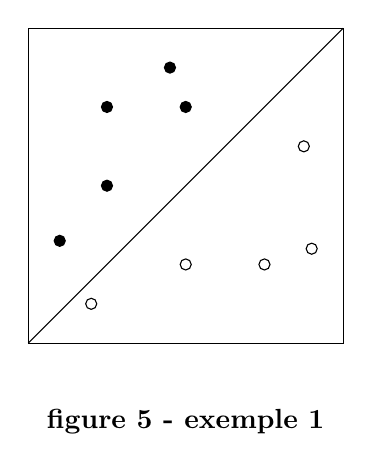
\begin{tikzpicture}[]
	%\draw[help lines, thick] (0,0) grid (4,4);
	\draw (0,0) rectangle (4,4);
	\filldraw (1,3) circle (2pt);
	\filldraw (2,3) circle (2pt);
	\filldraw (1,2) circle (2pt);
	\filldraw (0.4,1.3) circle (2pt);
	\filldraw (1.8,3.5) circle (2pt);
	\draw (0,0) -- (4,4);
	\filldraw (2,1) [fill=white] circle (2pt);
	\filldraw (3,1) [fill=white] circle (2pt);
	\filldraw (3.5,2.5) [fill=white] circle (2pt);
	\filldraw (3.6,1.2) [fill=white] circle (2pt);
	\filldraw (0.8,0.5) [fill=white] circle (2pt);
	\draw (2,-1) node { \textbf{figure 5 - exemple 1} };
\end{tikzpicture}
\end{center}
\vfill


Pour cela nous allons introduire un réseau de neurone composé d'une unité de type Sigmoid.
Ce neurone aura pour entrées les coordonnées du point choisi et pour sortie la valeur de la fonction d'activation qui est définie comme suit: 
\[ f(u,v) = \dfrac{1}{1+e^{-w_{1}u-w_{2}v+\theta}}. \]

\vfill
\begin{center}
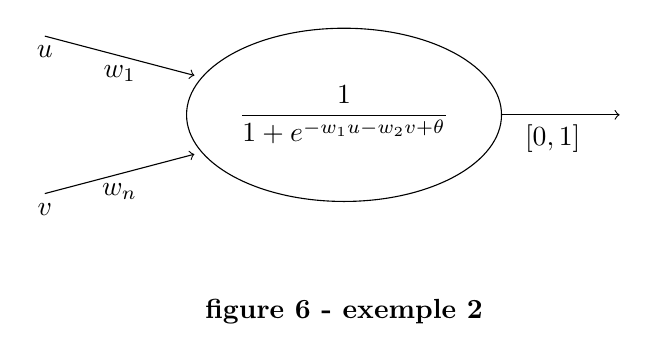
\begin{tikzpicture}[]
	%\draw[help lines, thick] (0,0) grid (9,5);
	\draw[->] (6.5,2.5)-- node[below, align=center] {$\left[0,1\right]$} (7.8,2.5)-- (8,2.5);
	\draw[->] (0.7,3.5) node [below] {$u$} -- node [below] {$w_{1}$} (2.6,3);
	\draw[->] (0.7,1.5) node [below] {$v$}-- node [below] {$w_{n}$} (2.6,2);
	\draw (4.5,2.5) node {$ \dfrac{1}{1+e^{-w_{1}u-w_{2}v+\theta}}  $} circle [x radius= 2, y radius=1.1];
	\draw (4.5,0) node { \textbf{figure 6 - exemple 2} };
\end{tikzpicture}
\end{center}
\vfill

Soit la fonction $\Phi_{x}(w_{1},w_{2},\theta)= \dfrac{1}{1+e^{-w_{1}u-w_{2}v+\theta}}$ avec $x=(u,v)$.\\

Soit $E$ un ensemble de triplets de la forme : 
$x = (u,v,p)$ 	avec $u$ et $v$ l'abscisse et l'ordonnée du point $x$ et $p$ sa position par rapport à la droite $d$.

	\[ \begin{cases} 0 &\mbox{Si  p est en dessous de d } \\
				 0.5 & \mbox{Si p est sur d } \\
				 1 & \mbox{Si p est au dessus de d }
	 		 \end{cases} \] \\
	 		 
Soit $ C_x(w_{1},w_{2},\theta) = \frac{1}{2}(y(x)-\Phi_x(w_{1},w_{2},\theta))^{2} $ la fonction de coût avec $y(x)=p$. Il suffit ensuite de minimiser le gradient de la fonction $\gamma$, décrite précédemment, afin d'obtenir les poids et inclinaison pour lesquelles le réseau $N$ nous donne des valeurs de position par rapport à la droite $d$, par interpolation sur les triplets de $E$.\\
%************************************************** fin de l'exemple *****************************************************************
\newline

%faire l'exemple avec le neuronne et la droite de point, et faire une transition avec la retropropagation
\subsection{Rétropropagation}
Nous avons vu dans la partie précédente, comment nous pouvons minimiser la fonction $\gamma$ à condition d'avoir son gradient. Le calcul du gradient devient très vite compliqué lorsque le réseau de neurone est formé de plusieurs couches de plusieurs neurones. Ce calcul est possible, néanmoins, grâce à la méthode de rétropropagation du gradient.

Avant de parler de la rétropropagation, nous devons introduire une nouvelle structure qui est le B-Diagramme (\textit{Backpropagation diagram}).
Ce diagramme représente les neurones utilisés dans notre réseau mais dans lesquelles nous stockons dans leurs partie gauche la valeur de la dérivée de leurs fonction et dans leurs partie droite la valeur de leurs fonction pour une entrée donnée.
\newline
% préciser les dérivéees partielle dans le diagramme
%************************************************** début de la figure *****************************************************************
%\vfill
\begin{center}
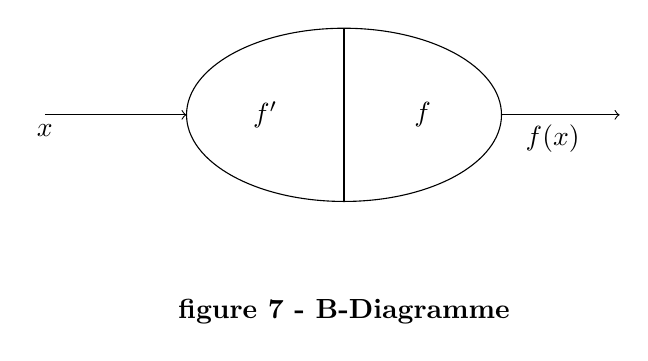
\begin{tikzpicture}[]
	%\draw[help lines, thick] (0,0) grid (9,5);
	\draw[->] (0.7,2.5) node [below] {$x$}-- (2.5,2.5);
	\draw[->] (6.5,2.5)-- node[below, align=center] {$f(x)$} (7.8,2.5)--(8,2.5);
	\draw (4.5,1.4)--(4.5,3.6);	
	\draw (4.5,2.5) circle [x radius= 2, y radius=1.1];
	\draw (3.5,2.5) node { $f'$ };
	\draw (5.5,2.5) node { $f$ };
	\draw (4.5,0) node { \textbf{figure 7 - B-Diagramme} };
\end{tikzpicture}
\end{center}
%\vfill
%************************************************** fin de la figure *****************************************************************
 
La rétropropagation se divise en deux étapes :
\begin{enumerate}
\item L'étape de \textit{feed-forward} : Cette étape consiste à parcourir notre réseau dans le sens direct afin de calculer pour chaque neurone, la valeur de sa fonction et de sa dérivée pour une valeur donnée. Une fois calculés, ces valeurs seront stockées dans chacun des neurones. Le résultat stocké à droite sera ensuite transmit au nœud suivant et le processus sera réitéré. % la régle avec leur et leurs
\item L'étape de rétropropagation : Dans cette étape le réseau sera parcouru dans le sens indirect et la valeur stockée à gauche sera utilisée, selon les cas suivants :
\begin{enumerate}
\item La composition  : Le réseau prend en entrée la constante 1. Celle-ci est multipliée par la valeur stockée dans la partie gauche du neurone. Le résultat sera ensuite transmis à l'unité suivante dans laquelle la constante sera multipliée par sa valeur de gauche. Le résultat final sera alors égale à $f'(g(x)).g'(x)$.
%************************************************** début de la figure *****************************************************************
\vfill
\begin{center}
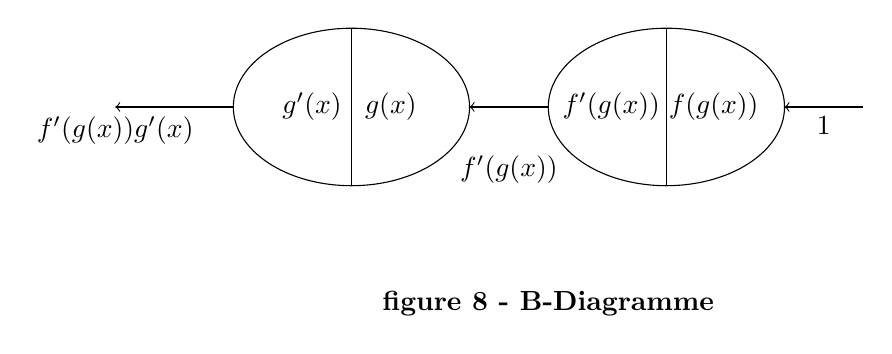
\begin{tikzpicture}[]
	%\draw[help lines, thick] (-1,0) grid (9,5);
	\draw[<-] (-1,2.5) node [below] {$f'(g(x))g'(x)$} -- (0.5,2.5);
	\draw[<-] (7.5,2.5)-- node [below] {$1$}(8.5,2.5);
	\draw[<-] (3.5,2.5) --(4.5,2.5);
	\draw (4,2) node [below] {$f'(g(x))$};
	\draw (2,3.5)--(2,1.5);
	\draw (6,3.5)--(6,1.5);
	\draw (2,2.5) circle [x radius= 1.5, y radius=1];
	\draw (6,2.5) circle [x radius= 1.5, y radius=1];
	\draw (1.5,2.5) node {$g'(x)$};
	\draw (2.5,2.5) node {$g(x)$};
	\draw (5.3,2.5) node {$f'(g(x))$};
	\draw (6.6,2.5) node {$f(g(x))$};
	\draw (4.5,0) node { \textbf{figure 8 - B-Diagramme} };
\end{tikzpicture}
\end{center}
\vfill
%************************************************** fin de la figure *****************************************************************
\item L'addition : Le réseau prend en entrée la constante 1, qui sera ensuite distribuée dans chaque unité. Lorsque deux unités se rencontre on additionne le résultat 
%************************************************** début de la figure *****************************************************************
\vfill
\begin{center}
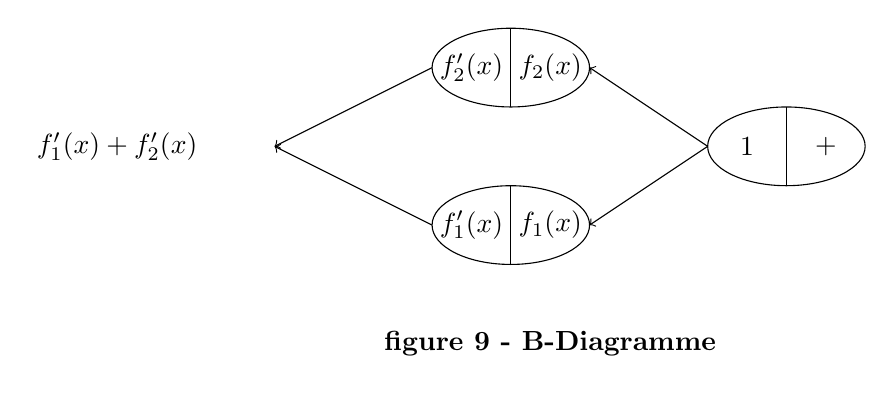
\begin{tikzpicture}[]
	%\draw[help lines, thick] (0,0) grid (9,5);
	\draw [<-] (5,1.5)--(6.5,2.5);
	\draw [<-] (5,3.5)--(6.5,2.5);
	\draw [->] (3,1.5)--(1,2.5);
	\draw [->] (3,3.5)--(1,2.5);
	\draw  (4,1)--(4,2);
	\draw  (4,3)--(4,4);
	\draw  (7.5,3)--(7.5,2);
	\draw (-1,2.5) node {$f'_{1}(x)+f'_2(x)$};
	\draw (3.5,1.5) node {$f'_{1}(x)$};
	\draw (3.5,3.5) node {$f'_2(x)$};
	\draw (4.5,1.5) node {$f_{1}(x)$};
	\draw (4.5,3.5) node {$f_2(x)$};
	\draw (8,2.5) node {$+$};
	\draw (7,2.5) node {$1$};
	\draw (4,1.5) circle [x radius= 1, y radius=0.5];
	\draw (4,3.5) circle [x radius= 1, y radius=0.5];
	\draw (7.5,2.5) circle [x radius= 1, y radius=0.5];
	\draw (4.5,0) node { \textbf{figure 9 - B-Diagramme} };
\end{tikzpicture}
\end{center}
\vfill
\newpage
%************************************************** fin de la figure *****************************************************************
\item Les entrées avec poids :
%\vfill
\begin{center}
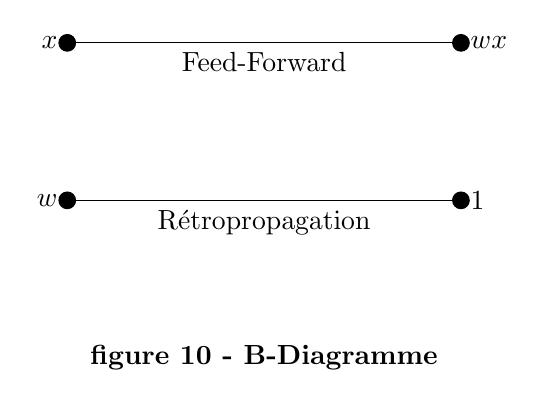
\begin{tikzpicture}[]
	%\draw[help lines, thick] (0,0) grid (9,5);
	\filldraw (2,2)[fill=black] circle (3pt);
	\draw (2,2)[left] node {$w$};
	\filldraw (7,2) [fill=black] circle (3pt);
	\draw (7,2)[right] node {$1$};
	\draw (2,2)--(7,2);
	\filldraw (2,4) [fill=black] circle (3pt);
	\draw (2,4)[left] node {$x$};
	\filldraw (7,4) [fill=black] circle (3pt);
	\draw (7,4)[right] node {$wx$};
	\draw (4.5,2) node [below] {Rétropropagation};
	\draw (4.5,4) node [below] {Feed-Forward};
	\draw (2,4)--(7,4);
	\draw (4.5,0) node { \textbf{figure 10 - B-Diagramme} };
\end{tikzpicture}
\end{center}
%\vfill
\end{enumerate}
\end{enumerate}
\section{Résolution de QBF-SAT}
Dans la partie précédente nous avons vu comment le processus d'apprentissage fonctionne. Dans cette partie, nous allons voir comment nous pouvons entrainer un réseau de neurone afin que celui-ci puisse résoudre des formules booléennes quantifiées.
Afin qu'un réseau de neurone puisse résoudre une formule QBF, il faut que celle-ci soit mise sous forme prénexe.
\subsection{Définition : Forme prénexe}
	On dit que une formule et sous forme prénexe si tout ses quantificateurs existentiels et universels sont placés au début de la formule. 
	\[ G= Q_{1}x_{1}Q_{2}x_{2}....Q_{n}x_{2}G' \] avec $G'$ une formule booléenne sans quantificateur.
\newline
\subsection{Définition : Forme Normale Conjonctive (CNF)}
Soit $F$ une formule booléenne et $(C_i)_{1\leq i \leq n}$ une famille de clauses telles que
\[F = C_1\land C_2 \land ... \land C_n\]
On dit alors que F est sous forme normale conjonctive.

\subsection{Format QDimacs}
Le format standard QDimacs permet de décrire des formules booléennes quantifiées qui sont prénexes et sous forme normale conjonctive. Il est compatible avec le format standard Dimacs des SAT-\textit{solver}.\\

La première ligne d'un fichier de type QDimacs est toujours de la forme "p cnf $v$ $c$" où $v$ est le nombre de variables et $c$ le nombre de clauses que contient la formule. Les variables étant numérotées de $1$ à $v$.\\

Le fichier contient ensuite un nombre potentiellement nul de lignes, se terminant par $0$, et décrivant l'ordre et la nature des quantificateurs. Une telle ligne définit des variables quantifiées existentiellement si elle commence par le caractère $e$, et universellement si elle commence par $a$.\\
Toute variable qui n'apparait dans aucune de ces ligne est supposée quantifiée existentiellement au tout début de la formule.\\

Les lignes suivantes du fichier décrivent les clauses de la formule une à une. Chaque ligne se termine par $0$ et liste toutes les variables de la clause, les variables sont négatives si elles apparaissent niées dans la clause, et positives sinon.\\
 
\textbf{Exemple de fichier en format QDimacs :}
\begin{framed}
\texttt{\\
p cnf 5 2\\ 
	a 1 4 0\\
	e 3 0\\
	a 2 0\\
	1 -2 4 0\\
	-3 4 5 0
}
\end{framed}
Ce fichier décrit la formule suivante : 
\[\exists x_5 \forall x_1 \forall x_4 \exists x_3 \forall x_2 \quad (x_1 \land \neg x_2 \land x_4 ) \lor (\neg x_3 \land x_4 \land x_5)\] 


\subsection{Choix des réseaux de neurones}
Pour résoudre une formule on utilisera deux réseaux qui s'affronteront dans un jeu. Un réseau représentera les quantificateurs universels et l'autre représentera les quantificateurs existentiels. Celui qui représentera les quantificateurs universels aura pour but de choisir des valuations qui permettront de rendre la formule fausse. Le réseau qui représentera les quantificateur existentiels aura pour but de choisir des valuations qui permettront de rendre vraie la formule. Au fur et mesure de l'exécution de l'algorithme, le pourcentage de victoires du réseau existentiel tendra vers $0\%$ si la formule est fausse et vers $100\%$ si elle est vraie. Les deux réseaux de neurone auront la même structure.\\
La taille de l'entrée du réseau de neurone est le nombre de variables de la formule donnée.
\newpage

Leur structure est donnée par le schéma suivant pour une formule :\\

%% Exprime le réseau de neurone qu'on a 
\begin{center}
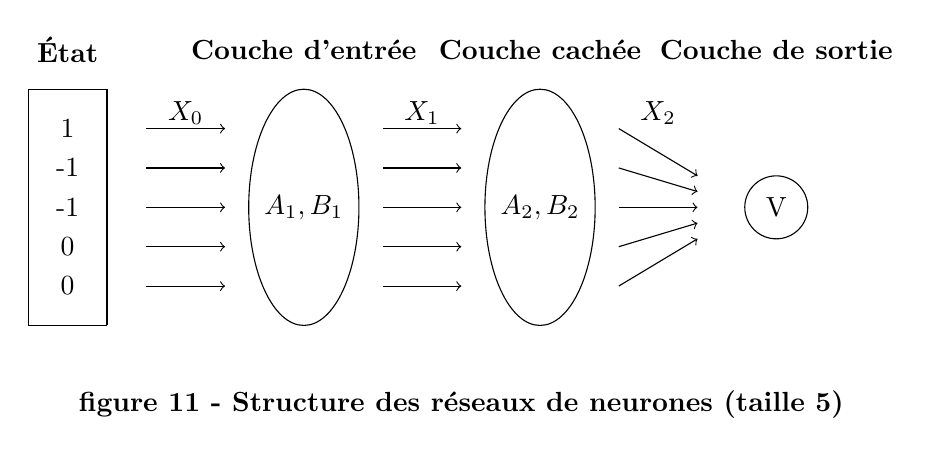
\begin{tikzpicture}[]
	%\draw[help lines, thick] (0,0) grid (11,5);
	\draw (3.5,2.5) node {$A_1,B_1$} circle [x radius=.7, y radius=1.5];
	\draw (6.5,2.5) node {$A_2,B_2$} circle [x radius=.7, y radius=1.5];
	\draw (9.5,2.5) node {V} circle [x radius=0.4, y radius=0.4];
	\draw [->] (1.5,1.5)--(2.5,1.5);
	\draw [->] (1.5,2)--(2.5,2);
	\draw [->] (1.5,2.5)--(2.5,2.5);
	\draw [->] (1.5,3)--(2.5,3);
	\draw [->] (1.5,3.5)--(2.5,3.5);
	\draw [->] (4.5,1.5)--(5.5,1.5);
	\draw [->] (4.5,2)--(5.5,2);
	\draw [->] (4.5,2.5)--(5.5,2.5);
	\draw [->] (4.5,3)--(5.5,3);
	\draw [->] (4.5,3.5)--(5.5,3.5);
	\draw [->] (7.5,1.5)--(8.5,2.1);
	\draw [->] (7.5,2)--(8.5,2.3);
	\draw [->] (7.5,2.5)--(8.5,2.5);
	\draw [->] (7.5,3)--(8.5,2.7);
	\draw [->] (7.5,3.5)--(8.5,2.9);
	\draw (0,4)--(1,4);
	\draw (0,4)--(0,1); 
	\draw (1,4)--(1,1); 
	\draw (0,1)--(1,1);
	\draw (0.5,3.5) node{1};
	\draw (0.5,3) node{-1};
	\draw (0.5,2.5) node{-1};
	\draw (0.5,2) node{0};
	\draw (0.5,1.5) node{0};
	\draw (.5,4.5) node {\textbf{État}}; 
	\draw (2,3.7) node {\textbf{$X_0$}}; 
	\draw (5,3.7) node {\textbf{$X_1$}}; 
	\draw (8,3.7) node {\textbf{$X_2$}}; 
	\draw (3.5,4.5) node {\textbf{Couche d'entrée}}; 
	\draw (6.5,4.5) node {\textbf{Couche cachée}}; 
	\draw (9.5,4.5) node {\textbf{Couche de sortie}}; 
	\draw (5.5,0) node { \textbf{figure 11 - Structure des réseaux de neurones (taille 5)}};
\end{tikzpicture}
\end{center}

Chaque réseau de neurone prend, en entrée, un état particulier du jeu (représentant une valuation partielle) et renvoie sa valeur $V\in[0,1]$.\\
Chaque neurone d'une couche de intermédiaire calcule l'image par la fonction sigmoïde d'une somme linéaire pondérée avec inclinaison de ses entrées. La transformation effectuée par la couche $i+1$ se traduit donc par :
\[ X_{i+1} = S(A_{i+1}X_i+B_{i+1}) \]
où :
\begin{enumerate}
\item[-] $X_i$ : vecteur reçu en entrée de couche
\item[-] $X_{i+1}$ : vecteur obtenue en sortie de couche
\item[-] $S$ : calcule l'image coordonnée par coordonnée du vecteur $A_{i+1}X_i+B_{i+1}$ par la fonction sigmoïde
\item[-] $A_{i+1}$ : matrice des poids
\item[-] $B_{i+1}$ : vecteur d'inclinaison
\end{enumerate}
La matrice des poids de la couche d'entrée est une matrice carrée, celle de la couche cachée est une matrice ligne.
\subsection{Description formelle de l'algorithme}
	\begin{algorithm}
	\caption{Deep QBF-SAT solver}
	\begin{algorithmic}
	\REQUIRE  $k$ 
	\WHILE{$ cmp < k$}
	\STATE  s, r = result(session())
	\STATE  us, uv, es, ev = build(s, r);
	\STATE store(us, uv, es, ev);
	\STATE train(uni, uniMset, uniMval);
	\STATE train(exi, exiMset, exiMval);
	\STATE $cmp++$;
	\ENDWHILE
	\end{algorithmic}
	\end{algorithm}
	L'algorithme consiste, pendant un nombre d'itérations donné $k$, à faire s'affronter les deux réseaux de neurones dans le cadre du jeu existentiel/universel décrit précédemment. À chaque itération, on recueille de nouvelles données d'expérience pour chacun des réseaux. On les ajuste selon le résultat de la partie puis on les rajoute aux données d'entrainement qu'on utilise pour le processus d'apprentissage.
	Les différentes étapes de chaque itération sont les suivantes :
	\begin{enumerate}
	\item \textbf{session:} calcule une session du jeu existentiel/universel et renvoie une matrice contenant la valuation choisie et les valeurs renvoyées par les réseaux de neurones pour chacun des choix
	\item \textbf{result:} prend en entrée une session et renvoie un couple $(s,v)$ où $s$ correspond à ladite session et $r$ correspond à la valeur de vérité de la formule pour la valuation contenue dans s et leau session
	\item \textbf{build:} prend en entrée le couple $(s,v,r)$ et renvoie les données d'expérience $us,uv$ pour le réseau \textit{UNI} et $es,ev$ pour le réseau \textit{EXI}, $us$ et $es$ contiennent les états rencontrés par les deux réseaux, $uv$ et $ev$ contiennent les nouvelles valeurs cibles pour la phase d'apprentissage
	\item \textbf{store:} prend en entrée les données d'expérience $us,uv$ et $es,ev$ et les enregistre respectivement dans les données d'apprentissage $uniMset, uniMval$ et $exiMset, exiMval$  
	\item \textbf{train:} effectue la phase d'apprentissage pour chacun des réseaux en utilisant les données d'apprentissage $uniMset, uniMval$ et $exiMset, exiMval$ 
	\end{enumerate}	 
\newpage	
\section{Langage Lua et Torch}
Le programme que nous avons décrit plus haut a été implémenté à l'aide d'un langage de script s'appelant Lua. Dans cette partie nous allons parler de ce langage de script et de sa librairie Torch spécialement conçue pour le domaine du "machine learning" 
	\subsection{Lua}
	Lua est un langage de script développé par une équipe de chercheurs brésiliens de l'Université pontificale Catholique de Rio de Janeiro.
	Sa réputation de langage portable est due au fait qu'il a été conçu en C. Ceci, permet à tout programme écrit en Lua d'être interprété dans une machine possédant le compilateur standard du langage C.
En plus d'être portable, Lua est aussi reconnu pour être facilment utilisable avec d'autre langage tel que le Java, C\#, Fortan ou bien d'autre langage de script tel que le Perl ou le Ruby.
Ce puissant langage étant rapide et léger a pu donné naissance à une librairie conçu pour le machine learning s'appelant Torch.
	
	\subsection{Torch}
	Torch comme dit précédement est une librairie d'algorithme scientifique du langage Lua conçu pour le machine learning. Cette librairie, permet d'avoir accés aux outils nécéssaire à l'utilisation de l'apprentissage profond. Elle offre une implémentation efficace et simple d'utilité des réseaux de neuronnes ainsi que tout les algorithme d'optimisation. Cette librarie doit sa popularité à la rapidité et la portabilité du langage Lua.

%% peut être un exemple de code concret ?  

\newpage 

\section{Conclusion}

\newpage

\section{Bibliographie}
  
\end{document}
